\documentclass{article}

\usepackage[utf8]{inputenc}
\usepackage{amsmath}
\usepackage{amsfonts} 
\usepackage{natbib}
\usepackage{graphicx}
\usepackage[lastexercise]{exercise}
\usepackage{geometry}
 \geometry{
 a4paper,
 total={170mm,257mm},
 left=20mm,
 top=20mm,
 }
%
%---------------------------------------------------------------------------------------------------------
%
\title{Lecture Notes on Copula}
\author{Giovanni Della Lunga}
\date{April 2018}
%
%---------------------------------------------------------------------------------------------------------
%
\begin{document}
\maketitle
%
%---------------------------------------------------------------------------------------------------------
%
\section{Introduction}
 
 Many real-life situations can be modelled by a large number of random variables which play a significant role, and such variates are generally not independent.  Therefore, it is often of fundamental importance to be able to link the marginal distributions of different variables in order to give a flexible and accurate descrip- tion of the joint law of the variables of interest. 	Copulas were introduced in 1959 in the context of probabilistic metric spaces and later exploited as a tool for understanding relationships among multivariate outcomes. 

A copula is a function that links univariate marginals to their joint multivariate distribution in such a way that it captures the entire dependence structure in the multivariate distribution. The main advantage provided by a copula-approach in dependence modelling is that the selection of an appropriate model for the dependence between variables X and Y , represented by the copula, can proceed independently from the choice of the marginal distributions. The seminal result in the history of copulas is due to Sklar that introduced in 1959 the notion, and the name, of copula, and proved the theo- rem that now bears his name (Sklar, 1959). The latter states that any multivariate distribution can be expressed as its copula function evaluated at its marginal distribution functions. Moreover, any copula function when evaluated at any marginal distributions is a multivariate distribution.
%
%---------------------------------------------------------------------------------------------------------
%
\section{Joint Cumulative Distribution Function }
Remember that the <b>joint cumulative function</b> of two random variables $X$ and $Y$ is defined as
\begin{align}%\label{}
\nonumber F_{XY}(x,y)=P(X \leq x, Y \leq y).
\end{align}
The joint CDF satisfies the following properties:

\begin{enumerate}
  \item  $F_X(x)=F_{XY}(x, \infty)$, for any $x$ (marginal CDF of $X$);
	\item  $F_Y(y)=F_{XY}(\infty,y)$, for any $y$ (marginal CDF of $Y$);
  \item  $F_{XY}(\infty, \infty)=1$;
  \item  $F_{XY}(-\infty, y)=F_{XY}(x,-\infty)=0$;
	\item 
   $\mathbb{P}(x_1 < X \leq x_2, \hspace{5pt} y_1  <Y \leq y_2)=$
     $F_{XY}(x_2,y_2)-F_{XY}(x_1,y_2)-F_{XY}(x_2,y_1)+F_{XY}(x_1,y_1)$;
	
  \item if $X$ and $Y$ are independent, then $F_{XY}(x,y)=F_X(x)F_Y(y)$.
\end{enumerate}

\noindent In particular from property 5, putting $x_2 \rightarrow +\infty$ and $y_2 \rightarrow +\infty$ we have

\begin{align}
\mathbb{P}(x_1 < X \leq +\infty, \hspace{5pt} y_1  <Y \leq +\infty) & =
     F_{XY}(+\infty,+\infty)-F_{XY}(x_1,+\infty)-F_{XY}(+\infty,y_1)+F_{XY}(x_1,y_1) \\
& = 1 - F_X(x) - F_Y(y) + F_{XY}(x_1,y_1)     
\end{align}
If we denote with 

\begin{equation}
\bar F_{XY}(x, y ) = \mathbb{P}[X > x, Y > y]
\end{equation}
we finally obtain

\begin{equation}
\bar F_{XY}(x, y ) = 1 - F_X(x) - F_Y(y) + F_{XY}(x, y)
\end{equation}
%
%---------------------------------------------------------------------------------------------------------
%
\section{Survival Copula}
The survival copula associated with the copula $C$ is

\begin{equation}
\bar C (u, v) = u + v - 1 + C(1-u, 1-v)
\end{equation}

It is easy to verify that $\bar C$ ha the copula properties. Once computed in $(1-u , 1-v)$ is equivalent to the complementary distribution function of a bivariate uniform distribution, since

\begin{align}
\bar C (1-u, 1- v) & = 1 - u + 1 - v - 1 + C(u, v) \\
& = 1 - \mathbb{P} (U_1 \le u) + 1 - \mathbb{P} (U_2 \le v) - 1 + \mathbb{P} (U_1 \le u, U_2 \le v) \\
& = 1 - \mathbb{P} (U_1 \le u) - \mathbb{P} (U_2 \le v) + \mathbb{P} (U_1 \le u, U_2 \le v) \\
& = \mathbb{P} (U_1 > u, U_2 > v)
\end{align}
%
%---------------------------------------------------------------------------------------------------------
%
\section{Copula and Measure}

If $C$ is absolutely continuous then it can be written in the form 

\begin{equation}
C(\mathbf{u}) = \int\limits_{[0, \mathbf{u}]^d} c(\mathbf{s}) \> d \mathbf{s}
\end{equation}
where $c$ is a suitable function called density of $C$. In particular, for almost all $\mathbf{u} \in \mathbb{I}^d$ one has

\begin{equation}
c(\mathbf{u}) = \frac{\partial^d C(\mathbf{u})}{\partial u_1 \dots \partial u_d}
\end{equation}
As stressed by many authors, this equation is far from obvious. In fact, there are some facts that are implicitly used: first, the mixed partial derivatives of order $d$ of $C$ exist and are equal almost everywhere on $\mathbb{I}^d$; second each mixed partial derivative is actually almost everywhere equal to the density $c$. We will use this result to formally define a measure induced on $\mathbb{I}^d$ by $C$. 

\begin{equation}
dC(\mathbf{u}) = c(\mathbf{u}) \> d \mathbf{u}
\end{equation}
In particular for a bivariate copula we have

\begin{equation}
dC(u, v) = \frac{\partial^2 C(u, v)}{\partial u \partial v} du dv
\end{equation}
%
%---------------------------------------------------------------------------------------------------------
%
\section{Density Function for the Sum of Correlated Gaussian Variables}

When two random variables are independent, the probability density function for their sum is the
convolution of the density functions for the variables that are summed. We consider here the case
when these two random variables are correlated. Let $x$ and $y$ be the two correlated random variables,
and $z = x + y$. The standard procedure for obtaining the distribution of a function $z = g(x,y)$ is to
integrate the joint density function $p_{xy}(x,y)$ over the region $D$ of the $xy$ plane where $g(x,y) < Z$ to
obtain the cumulative distribution $P_z(Z)$. This is then differentiated with respect to $Z$ to obtain the
density function $p_z(z)$. The cumulative distribution is:

\begin{equation}
    P_z(Z)= \int\int\limits_D \> p_{xy}(x,y) \>dx \>dy
\end{equation}

In some cases, $D$ may be disjoint, but for $z = x + y$ it is just the area under that line. When $x$ and $y$ are
independent, the joint density function separates into a product of the two marginal density functions
$p_x(x)$ and $p_y(y)$, and the procedure we are about to describe, along with $y = z - x$, leads directly to the
convolution:

\begin{equation}
    \begin{split}
        & P_z(Z) = \int\limits_{-\infty}^{+\infty} \Biggl( \int\limits_{-\infty}^{Z-x} p_x(x)p_y(y) \> dy \Biggr) \> dx \\
        & p_Z(z) = \frac{dP_z(Z)}{dZ} = \int\limits_{-\infty}^{+\infty} p_x(x)p_y(z-x) \> dx
    \end{split}
\end{equation}
Since we are considering $x$ and $y$ to be correlated, we must retain the joint density function itself:

\begin{equation}
    \begin{split}
        & P_z(Z) = \int\limits_{-\infty}^{+\infty} \Biggl( \int\limits_{-\infty}^{Z-x} p_{xy}(x, y) \> dy \Biggr) \> dx \\
        & p_Z(z) = \frac{dP_z(Z)}{dZ} = \int\limits_{-\infty}^{+\infty} p_{xy}(x, z-x) \> dx
    \end{split}
\end{equation}
using the Leibnitz rule for the derivation of integrals. 

The failure of the joint density function to separate results in $p_z(z)$ no longer having the form of a
convolution. To illustrate this we consider the Gaussian case. The joint density function for Gaussian
$x$ and $y$ coupled through a correlation coefficient $\rho$ is

\begin{equation}
    p(x,y) = \frac{\exp{\Bigl[-\frac{1}{2(1-\rho^2)}
                        \Bigl(
                            \frac{(x-\bar x)^2}{\sigma_x^2} +
                            \frac{(y-\bar y)^2}{\sigma_y^2} -
                            \frac{2\rho(x-\bar x)(y-\bar y)}{\sigma_x \sigma_y}
                        \Bigr) \Bigr]
                        }
                  }
    {2\pi \sigma_x \sigma_y \sqrt{1-\rho^2}}
\end{equation}
where we dont't assume that either $x$ or $y$ is zero-mean. The computation of the integral is extremely tedious but trivial. First of all let's re-write the argument of the exponential function using the following change of variables:
\begin{equation}
    z = x + y \Rightarrow y = z - x, \quad \bar y = \bar z - \bar x \Rightarrow (y - \bar y) = (z -\bar z) - (x - \bar x)
\end{equation}
and we obtain
\begin{equation}
    \begin{split}
        &
        \frac{(x-\bar x)^2}{\sigma_x^2} +
        \frac{(y-\bar y)^2}{\sigma_y^2} -
        \frac{2\rho(x-\bar x)(y-\bar y)}{\sigma_x \sigma_y} \\
        & =
        \frac{\sigma^2_y (x-\bar x)^2 + \sigma^2_x [(z-\bar z) - (x -\bar x)]^2 - 2 \rho \sigma_x \sigma_y (x - \bar x)[(z-\bar z) - (x -\bar x)]}
        {\sigma^2_x \sigma^2_y} \\
        & = \frac{1}{\sigma^2_x \sigma^2_y} 
        \Bigl\{
        \sigma^2_y(x-\bar x)^2 + \sigma^2_x(z-\bar z)^2 + \sigma^2_x(x-\bar x)^2 - 2 \sigma^2_x (z-\bar z)(x - \bar x) - \\
        & - 2 \rho \sigma_x \sigma_y (z - \bar z)(x - \bar x) + 2 \rho \sigma_x \sigma_y (x- \bar x)^2
        \Bigr\} \\
        & = \frac{1}{\sigma^2_x \sigma^2_y}
        \Bigl\{
        \sigma^2_z (x - \bar x)^2 + \sigma^2_x (z-\bar z)^2 -2(z-\bar z)(x-\bar x)(\sigma^2_x + \rho \sigma_x \sigma_y)
        \Bigr\}
    \end{split}
\end{equation}
where
\begin{equation}
    \sigma_z^2 = \sigma_x^2 + \sigma_y^2 + 2 \rho \sigma_x \sigma_y
\end{equation}
\begin{equation}
    \tilde x = x - \bar x, \quad \tilde z = z - \bar z
\end{equation}
performing the algebraic computation and rearranging terms inside braces we obtain
\begin{equation}
    \frac{1}{\sigma^2_x \sigma^2_y}
    \Bigl\{
        \sigma^2_z {\tilde x}^2 - 2 \tilde x \tilde z (\sigma^2_x + \rho \sigma_x \sigma_y ) + \sigma_x^2 {\tilde z}^2
    \Bigr\}
\end{equation}
Put
\begin{equation}
    \alpha = \Biggl[   
        \frac{\sigma^2_x + \rho \sigma_x \sigma_y}{\sigma_z}
    \Biggr]
\end{equation}
and re-write the previous term adding and subtracting the factor $\alpha^2 {\tilde z}^2$ (for simplicity we don't take into account for the moment the multiplicative factor $1/\sigma_x^2\sigma_y^2$)
\begin{equation}
    \begin{split}
        \sigma^2_z {\tilde x}^2 - 2 \tilde x \tilde z (\sigma^2_x + \rho \sigma_x \sigma_y ) + \sigma_x^2 {\tilde z}^2  & = \sigma^2_z {\tilde x}^2 - 2 \tilde x \tilde z (\sigma^2_x + \rho \sigma_x \sigma_y ) + \sigma_x^2 {\tilde z}^2 + \alpha^2 {\tilde z}^2 - \alpha^2 {\tilde z}^2 \\    
        & = \Biggl[ \sigma^2_z {\tilde x}^2 - 2 \tilde x \tilde z (\sigma^2_x + \rho \sigma_x \sigma_y ) +
        \frac{\bigl(\sigma_x^2 + \rho \sigma_x \sigma_y \bigr)^2}{\sigma^2_z} {\tilde z}^2 \Biggr] + \sigma^2_x {\tilde z}^2 - \alpha^2 {\tilde z}^2  \\
        & = \Bigl[ \sigma_z {\tilde x} - \alpha {\tilde z} \Bigr]^2 + \Bigl[\sigma_x^2 - \alpha^2 \Bigr] {\tilde z}^2 \\
        & = \sigma_z^2 \Bigl[ {\tilde x} - \frac{\alpha}{\sigma_z} {\tilde z} \Bigr]^2 + \Bigl[\sigma_x^2 - \alpha^2 \Bigr] {\tilde z}^2
    \end{split}
\end{equation}
Let's compute the second term
\begin{equation}
    \begin{split}
        (\sigma^2_x - \alpha^2) {\tilde z}^2 & = 
        \Biggl[
            \sigma^2_x - \frac{\sigma^4_x + \rho^2 \sigma^2_x \sigma^2_y + 2 \rho \sigma^3_x \sigma_y}{\sigma^2_z}
        \Biggr] {\tilde z}^2\\
        & = \Biggl[ 
                \frac{\sigma^2_x \sigma^2_z - \sigma^4_x - \rho^2 \sigma^2_x \sigma^2_y - 2 \rho \sigma^3_x \sigma_y}{\sigma^2_z} 
            \Biggr] {\tilde z}^2\\
        & = \frac{1}{\sigma^2_z} 
            \Biggl[
                (\sigma_x^2 + \sigma_y^2 + 2 \rho \sigma_x \sigma_y) \sigma^2_x  - \sigma^4_x - \rho^2 \sigma^2_x \sigma^2_y - 2 \rho \sigma^3_x \sigma_y
            \Biggr] {\tilde z}^2 \\
        & = \frac{1}{\sigma^2_z} 
            \Biggl[
                \sigma_x^4 + \sigma^2_y \sigma^2_x + 2 \rho \sigma^3_x \sigma_y
                - \sigma^4_x - \rho^2 \sigma^2_x \sigma^2_y - 2 \rho \sigma^3_x \sigma_y
            \Biggr] {\tilde z}^2 \\
        & = \frac{1}{\sigma^2_z} 
            \Biggl[
                (1-\rho^2)\sigma_x^2 \sigma_y^2
            \Biggr] {\tilde z}^2
    \end{split}
\end{equation}
This give us
\begin{equation}
    \sigma^2_z {\tilde x}^2 - 2 \tilde x \tilde z (\sigma^2_x + \rho \sigma_x \sigma_y ) + \sigma_x^2 {\tilde z}^2 = \sigma_z^2 \Bigl[ {\tilde x} - \frac{\alpha}{\sigma_z} {\tilde z} \Bigr]^2
    + \frac{1}{\sigma^2_z} 
            \Biggl[
                (1-\rho^2)\sigma_x^2 \sigma_y^2
            \Biggr] {\tilde z}^2
\end{equation}
Remember that we have to multiply by 
\begin{equation}
    -\frac{1}{2(1 - \rho^2) \sigma_x^2 \sigma_y^2}
\end{equation}
So, finally, the argument of the exponential function can be written as

\begin{equation}
    - \frac{\sigma^2_z}{2(1-\rho^2)\sigma^2_x\sigma^2_y} \Biggl( \tilde x - \frac{\alpha}{\sigma_z} \tilde z \Biggr)^2 - \frac{1}{2 \sigma^2_z} {\tilde z}^2
\end{equation}
and the integral can be written as 

\begin{equation}
    \begin{split}
        p_Z(z) & = \int\limits_{-\infty}^{+\infty} p_{xy}(x, z-x) \> dx \\
        & = \frac{1}{2\pi \sigma_x \sigma_y \sqrt{1-\rho^2}} 
        \int\limits_{-\infty}^{+\infty}
        \exp \Biggr[ 
        - \frac{\sigma^2_z}{2(1-\rho^2)\sigma^2_x\sigma^2_y} \Biggl( \tilde x - \frac{\alpha}{\sigma_z} \tilde z \Biggr)^2 - \frac{1}{2 \sigma^2_z} {\tilde z}^2
        \Biggr] \> dx \\
        & = \frac{1}{2\pi \sigma_x \sigma_y \sqrt{1-\rho^2}}
        \exp \Biggl[ - \frac{1}{2 \sigma^2_z} {\tilde z}^2 \Biggl]
        \int\limits_{-\infty}^{+\infty}
        \exp \Biggr[ 
        - \frac{\sigma^2_z}{2(1-\rho^2)\sigma^2_x\sigma^2_y} \Biggl( \tilde x - \frac{\alpha}{\sigma_z} \tilde z \Biggr)^2
        \Biggr] \> dx
    \end{split}
\end{equation}
using
\begin{equation}
    \begin{split}
        & \mu = \frac{\alpha}{\sigma_z}\tilde z \\
        & {\tilde \sigma}^2 = (1-\rho^2)\frac{\sigma^2_x\sigma^2_y}{\sigma^2_z} 
    \end{split}
\end{equation}
and
\begin{equation}
    \tilde \omega = \frac{\tilde x - \mu}{\tilde \sigma} \Rightarrow d \tilde \omega = \frac{1}{\tilde \sigma}d \tilde x = \frac{1}{\tilde \sigma}dx
\end{equation}
we can re-write the integral as
\begin{equation}
\int\limits_{-\infty}^{+\infty}
        \exp \Biggr[ 
        - \frac{\sigma^2_z}{2(1-\rho^2)\sigma^2_x\sigma^2_y} \Biggl( \tilde x - \frac{\alpha}{\sigma_z} \tilde z \Biggr)^2
        \Biggr] \> dx    =
        {\tilde \sigma}
        \int\limits_{-\infty}^{+\infty}
        \exp\bigl( -\frac{\omega^2}{2} \bigr) \> dw = \sqrt{2\pi} {\tilde \sigma}
\end{equation}
and
\begin{equation}
    \begin{split}
        p_Z(z) & = \int\limits_{-\infty}^{+\infty} p_{xy}(x, z-x) \> dx \\
        & = \frac{1}{2\pi \sigma_x \sigma_y \sqrt{1-\rho^2}}
        \exp \Biggl[ - \frac{1}{2 \sigma^2_z} {\tilde z}^2 \Biggl]
        \int\limits_{-\infty}^{+\infty}
        \exp \Biggr[ 
        - \frac{\sigma^2_z}{2(1-\rho^2)\sigma^2_x\sigma^2_y} \Biggl( \tilde x - \frac{\alpha}{\sigma_z} \tilde z \Biggr)^2
        \Biggr] \> dx \\
        & = \frac{1}{2\pi \sigma_x \sigma_y \sqrt{1-\rho^2}}
        \exp \Biggl[ - \frac{1}{2 \sigma^2_z} {\tilde z}^2 \Biggl] \Bigl( \sqrt{1-\rho^2} \Bigr)  \frac{\sigma_x \sigma_y}{\sigma_z}\sqrt{2\pi} \\
        & = \frac{1}{\sqrt{2\pi}\sqrt{\sigma_x^2 + \sigma_y^2 + 2 \rho \sigma_x \sigma_y}} \exp \Biggl[ - \frac{1}{2 \sigma^2_z} {\tilde z}^2 \Biggl] \\
        & = \frac{1}{\sqrt{2\pi (\sigma_x^2 + \sigma_y^2 + 2 \rho \sigma_x \sigma_y})}
        \exp\Biggl[
        -\frac{(z - (\bar x + \bar y))^2}{2(\sigma^2_x + \sigma_y^2 + 2 \rho \sigma_x \sigma_y)}
        \Biggr]
    \end{split}
\end{equation}
which is gaussian with
\begin{equation}
    \begin{split}
        & \bar z = \bar x + \bar y  \\
        & \sigma_z^2 = \sigma_x^2 + \sigma_y^2 + 2\rho \sigma_x \sigma_y
    \end{split}
\end{equation}
So the mean is unaffected by the correlation, but the variance is made larger or smaller according to whether the correlation is positive or negative, respectively. 
%
%---------------------------------------------------------------------------------------------------------
%
\section{On Hoeffding's Identity}

The Hoeffding's Identity can be written as

\begin{equation}
\text{cov}(X,Y)=\int_{\mathbb{R}\times\mathbb{R}}[F_{XY}(x,y)-F_X(x) F_Y(y)]\>dx\>dy 
\end{equation}
It is interesting, and quite important, actually, to understand that the covariance (or the correlation) can be seen as some ‘distance‘ to the independence. More precisely, observe that

\begin{equation}
\text{cov}(X,Y)=\int_{\mathbb{R}\times\mathbb{R}}[F_{XY}(x,y)-F_{X,Y}^\perp(x,y)]\>dx\>dy 
\end{equation}
where $F_{X,Y}^\perp(x,y)$  would be the joint cumulative distribution function of some independent variables, with the same marginal distributions.

Now, the thing is that the proof is not trivial! Let $I$ denote the indicator function, then we can write

\begin{equation}
    \begin{split}
        \int\limits_0^\infty [I(z\le u) - I(x\le u)] du & = \lim\limits_{\alpha \rightarrow \infty}
        \int\limits_0^\alpha [I(z\le u) - I(x\le u)] du \\
        & = \lim\limits_{\alpha \rightarrow \infty} \Bigl\{\int\limits_0^z I(z\le u) \> du + \int\limits_z^\alpha I(z\le u) \> du \\
        & - \int\limits_0^x I(x\le u) \> du - \int\limits_x^\alpha I(x\le u) \> du \Bigr\} \\
        & = \lim\limits_{\alpha \rightarrow \infty}
             \Bigl\{ \int\limits_z^\alpha 1 \> du - \int\limits_x^\alpha 1 \> du \Bigr\} \\
        & = \lim\limits_{\alpha \rightarrow \infty} [ \alpha - z - \alpha + x]  = x - z
    \end{split}
\end{equation}
Hence for $X_1, Y_1, X_2, Y_2 \ge 0$ we find

\begin{equation}
    \begin{split}
        (X_1 - X_2)(Y_1 - Y_2) & = \int_{\mathbb{R}\times\mathbb{R}} \Bigl[
        I(X_2\le u)I(Y_2\le v) + I(X_1\le u)I(Y_1\le v) \\
        & - I(X_2\le u)I(Y_1\le v) - I(X_1\le u)I(Y_2\le v) 
        \Bigr] \>du\>dv
    \end{split}
\end{equation}
Now take the expectation of both sides and invert the integral and the expectation in the right hand side of the equation
\begin{equation}
    \begin{split}
        \mathbb{E}[(X_1 - X_2)(Y_1 - Y_2)] & = \int_{\mathbb{R}\times\mathbb{R}} \Bigl[
        \mathbb{E}(I(X_2\le u)I(Y_2\le v)) + \mathbb{E}(I(X_1\le u)I(Y_1\le v)) \\
        & - \mathbb{E}(I(X_2\le u)I(Y_1\le v)) - \mathbb{E}(I(X_1\le u)I(Y_2\le v)) 
        \Bigr] \>du\>dv
    \end{split}
\end{equation}
Let $(X_1, Y_1)$ and $(X_2, Y_2)$ be independent identically distributed pairs, using the fact that

\begin{equation}
    \mathbb{E} [I(X \le u)] = \mathbb{P} (X \le u)
\end{equation}
we obtain

\begin{equation}
    \begin{split}
        \mathbb{E}[(X_1 - X_2)(Y_1 - Y_2)] & = \int_{\mathbb{R}\times\mathbb{R}} \Bigl[
        \mathbb{P}(X_2\le u, Y_2\le v) + \mathbb{P}(X_1\le u, Y_1\le v) \\
        & - \mathbb{P}(X_2\le u) \mathbb{P}(Y_1\le v) - \mathbb{P}(X_1\le u) \mathbb{P}(Y_2\le v) 
        \Bigr] \>du\>dv \\
        & = 2 \int_{\mathbb{R}\times\mathbb{R}} \Bigl[
            \mathbb{P}(X_1\le u, Y_1\le v) - \mathbb{P}(X_1\le u) \mathbb{P}(Y_1\le v)
        \Bigr] \>du\>dv \\
        & =  2 \int_{\mathbb{R}\times\mathbb{R}} \Bigl[
            F_{X_1, Y_1}(u, v) - F_{X_1}(u)F_{Y_1}(v)
        \Bigr] \>du\>dv
    \end{split}
\end{equation}
but

\begin{equation}
    \begin{split}
        \mathbb{E}[(X_1 - X_2)(Y_1 - Y_2)] & = \mathbb{E}[X_1Y_1 - X_1Y_2 - X_2Y_1 + X_2Y_2]   \\
        & = \mathbb{E}[X_1Y_1] - \mathbb{E}[X_1]\mathbb{E}[Y_2] - \mathbb{E}[X_2]\mathbb{E}[Y_1] + \mathbb{E}[X_2Y_2] \\
        & = 2\Bigl( \mathbb{E}[X_1Y_1] - \mathbb{E}[X_1]\mathbb{E}[Y_1] \Bigr) \\
        & = 2 \> \text{cov}(X_1,Y_1)
    \end{split}
\end{equation}
So we get Hoeffding's identity. This identity can be written using the definition of copula as

\begin{equation}
\text{cov}(X,Y)=\int_{\mathbb{R}\times\mathbb{R}}[C(F_X(x), F_Y(y))-F_X(x) F_Y(y)]\>dx\>dy 
\end{equation}
and taking into account the Fréchet inequality:

\begin{equation}
    \begin{split}
        & \int_{\mathbb{R}\times\mathbb{R}}[C^-(F_X(x), F_Y(y))-F_X(x) F_Y(y)]\>dx\>dy \le \text{cov}(X,Y) \\
        & \text{cov}(X,Y) \le \int_{\mathbb{R}\times\mathbb{R}}[C^+(F_X(x), F_Y(y))-F_X(x) F_Y(y)]\>dx\>dy 
    \end{split}
\end{equation}
where $C^-$ is the \textbf{minimum copula} and $C^+$ is the \textbf{maximum copula}. 
%
%---------------------------------------------------------------------------------------------------------
%
\section{Dependence Concepts}

Copulas provide a natural way to study and measure dependence between random variables. Copula properties are invariant under strictly increasing transformations of the underlying random variables. Linear correlation (or Pearson’s correlation) is most frequently used in practice as a measure of dependence. However, since linear correlation is not a copula-based measure of dependence, it can often be quite misleading and should not be taken as the canonical dependence measure. Below we recall the basic properties of linear correlation, and then continue with some copula based measures of dependence.

\subsection{Linear Correlation Coefficient}

\noindent \textbf{Definition}. Let $(X,Y)^T$ be a vector of random variables with nonzero finite variances. The linear correlation coefficient for $(X,Y)^T$ is
\begin{equation}
	\rho(X,Y) = \frac{Cov(X,Y}{\sqrt{Var(X)}\sqrt{Var(Y)}}
\end{equation}	
where $Cov(X,Y) = \mathbb{E}(XY) -\mathbb{E}(X)\mathbb{E}(Y)$ is the covariance of $(X,Y)^T$, and $Var(X)$ and
$Var(Y)$ are the variances of $X$ and $Y$.


Linear correlation is a popular but also often misunderstood measure of dependence. The popularity of linear correlation stems from the ease with which it can be calculated and it is a natural scalar measure of dependence in elliptical distributions (with well known members such as the multivariate normal and the multivariate t-distribution). However most random variables are not jointly elliptically distributed, and using linear correlation as a measure of dependence in such situations might prove very misleading. Even for jointly elliptically distributed random variables there are situations where using linear correlation, as defined by (??), does not make sense. We might choose to model some scenario using heavy-tailed distributions such as t2-distributions. In such cases the linear correlation coefficient is not even defined because of infinite second moments.

\bigskip
\noindent\textbf{Property}. $\rho(X,Y)$ is bounded:
$$
\rho_l \le \rho \le \rho_u
$$
where the bounds $\rho_l$ and $\rho_u$ are defined as
\begin{equation}
\begin{split}
& \rho_l = \frac{\iint_D \Bigl[ C^-(F_1(x), F_2(y)) - F_1(x)F_2(y) \Bigr] \> dx\>dy}
                        {\sqrt{
                                  \Bigl[ \int_{Dom(F_1)}(x-\mathbb{E}(x))^2dF_1(x) \Bigr]
                                  \Bigl[ \int_{Dom(F_2)}(y-\mathbb{E}(y))^2dF_2(y) \Bigr]
                                 }
                        } \\
& \rho_u = \frac{\iint_D \Bigl[ C^+(F_1(x), F_2(y)) - F_1(x)F_2(y) \Bigr] \> dx\>dy}
                        {\sqrt{
                                  \Bigl[ \int_{Dom(F_1)}(x-\mathbb{E}(x))^2dF_1(x) \Bigr]
                                  \Bigl[ \int_{Dom(F_2)}(y-\mathbb{E}(y))^2dF_2(y) \Bigr]
                                 }
                        } \\
\end{split}
\end{equation}
and are attained respectively when $X$ and $Y$ are countermonotonic and comonotonic.

\noindent\textbf{Proof}. The bound for $\rho(X,Y)$ can be obtained directly from Hoeffding's expression for covariance together with the Fréchet inequality. 
	
\bigskip	
\noindent\textbf{Example}. Let $X \sim LN(0, \sigma_1^2)$ and $Y \sim LN(0, \sigma_2^2)$. Then $\rho_{min} = \rho(e^{\sigma_1Z}, e^{-\sigma_2 Z})$ and $\rho_{max} = \rho(e^{\sigma_1Z}, e^{\sigma_2 Z})$, where $Z \sim N(0,1)$. $\rho_{min}$ and $\rho_{max}$ can be computed (see Exercise ...) yielding:

\begin{equation}
\begin{split}
& \rho_l = \frac{exp(-\sigma_1 \sigma_2) - 1}
                        {
                         \sqrt{(exp(\sigma_1^2) - 1)}
                         \sqrt{(exp(\sigma_2^2) - 1)}
                        } \le 0 \\
& \rho_u = \frac{exp(\sigma_1 \sigma_2) - 1}
                        {
                         \sqrt{(exp(\sigma_1^2) - 1)}
                         \sqrt{(exp(\sigma_2^2) - 1)}
                        } \ge 0
\end{split}
\end{equation}
from which follows that
$$
\lim\limits_{\sigma \rightarrow \infty} \rho_{min} =\lim\limits_{\sigma \rightarrow \infty} \rho_{max}=0  
$$

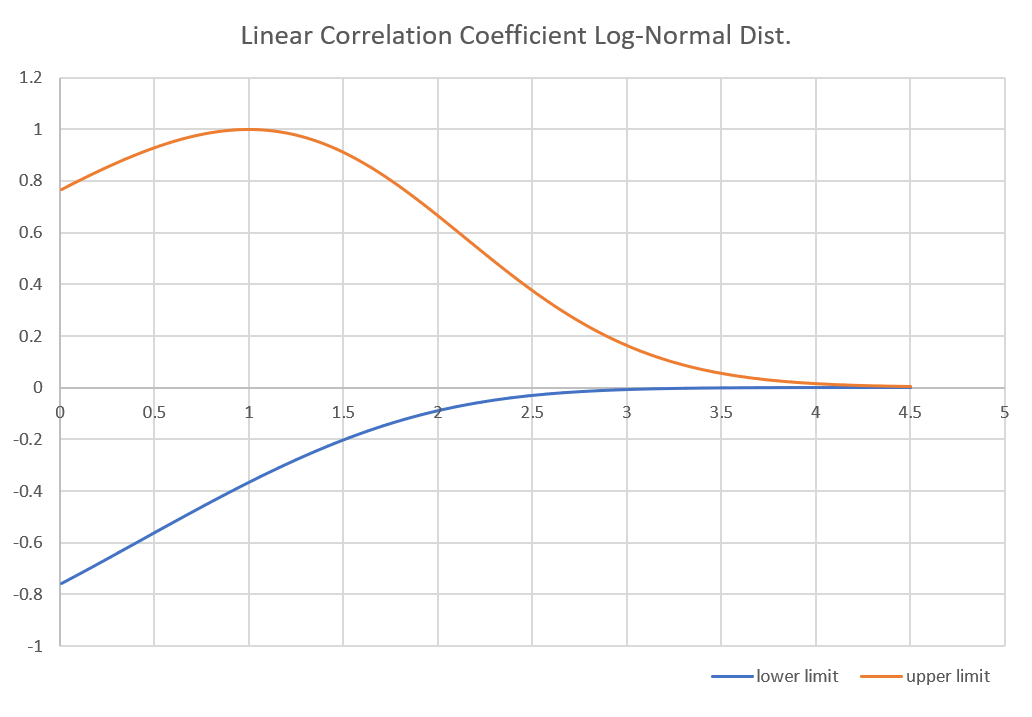
\includegraphics[scale=.75]{fig/linear_correlation_lognormal.png} 

\subsection{Concordance}

Concordance concepts, loosely speaking, aim at capturing the fact that the probability of having "large" (or "small") values of both $X$ and $Y$ is high, while the probability of having "large" values of $X$ together with "small" values of "Y" - or viceversa - is low.


Let $(x, y)^T$ and $(\tilde x, \tilde y)^T$ be two observations from a vector $(X, Y )^T$ of continuous random variables. Then $(x, y)^T$ and $(\tilde x, \tilde y)^T$ are said to be concordant if $(x-\tilde x)(y-\tilde y) > 0$, and discordant if $(x-\tilde x)(y-\tilde y) < 0$.


The following theorem can be found in Nelsen (1999) p. 127. Many of the results in this section are direct consequences of this theorem.

\textbf{Theorem}. Let $(X, Y )^T$ and $(\tilde X, \tilde Y )^T$ be independent vectors of continuous random variables with joint distribution functions $H$ and $\tilde H$, respectively, with common margins $F$ (of $X$ and $\tilde X$) and $G$ (of $Y$ and $\tilde Y$). Let $C$ and $\tilde C$ denote the copulas of $(X, Y )^T$ and $(\tilde X, \tilde Y )^T$ respectively,so that $H(x,y)=C(F(x),G(y))$ and $\tilde H(x,y)= \tilde C(F(x),G(y))$. Let $Q$ denote the difference between the probability of concordance and discordance of $(X, Y )^T$ and $(\tilde X, \tilde Y )^T$ , i.e. let

\begin{equation}
	Q=\mathbb{P}[(X-\tilde X)(Y-\tilde Y) > 0]-\mathbb{P}[(X-\tilde X)(Y-\tilde Y) < 0] 
\end{equation}

Then

\begin{equation}
	Q=Q(C, \tilde C) = 4 \iint\limits_{[0,1]^2} \tilde C (u,v) dC(u,v) -1
\end{equation}

\textbf{Proof}. Since the random variables are all continuous,
$$
\mathbb{P}[(X-\tilde X)(Y-\tilde Y) < 0] = 1 -\mathbb{P}[(X-\tilde X)(Y-\tilde Y) > 0] \Rightarrow Q = 2 
\mathbb{P}[(X-\tilde X)(Y-\tilde Y) > 0] - 1
$$
But
$$
\mathbb{P}[(X-\tilde X)(Y-\tilde Y) > 0] = \mathbb{P}[X > \tilde X, Y > \tilde Y] + \mathbb{P}[X <\tilde X, Y < \tilde Y]
$$
and these probabilities can be evaluated by integrating over the distribution of one of the vectors $(X, Y)^T$ or $(\tilde X, \tilde Y)^T$. Hence

\begin{align}
\mathbb{P}[X > \tilde X, Y > \tilde Y] & = \mathbb{P}[ \tilde X < X, \tilde Y < Y] \\
& = \iint\limits_{\mathbb{R}^2} \mathbb{P}[ \tilde X < x, \tilde Y < y] \> dC[F(x), G(y)] \\
& = \iint\limits_{\mathbb{R}^2} \tilde C [F(x), G(y)]  \> dC[F(x), G(y)]
\end{align}
Employing the probability-integral transform $u=F(x)$ and $v = G(y)$ then yields

\begin{equation}
\mathbb{P}[X > \tilde X, Y > \tilde Y] = \mathbb{P}[ \tilde X < X, \tilde Y < Y] 
= \iint\limits_{[0, 1]^2} \tilde C(u, v)  \> dC(u, v)
\end{equation}
Similarly,

\begin{align}
\mathbb{P}[X < \tilde X, Y < \tilde Y] & = \iint\limits_{\mathbb{R}^2} \mathbb{P}[ \tilde X > x, \tilde Y > y] \> dC[F(x), G(y)] \\
& = \iint\limits_{\mathbb{R}^2} \bigl\{1 - F(x) - G(y) + \tilde C[F(x), G(y)]    \bigr\}  \> dC[F(x), G(y)] \\
& = \iint\limits_{[0, 1]^2} \bigl\{1 - u - v + \tilde C(u, v)   \bigr\}  \> dC(u, v)
\end{align}
But since $C$ is the joint distribution function of a vector $(U, V)^T$ of $U(0, 1)$ random variables, $\mathbb{E}(U) = \mathbb{E}(V) = 1/2$, and hence

\begin{equation}
\mathbb{P}[X < \tilde X, Y < \tilde Y] = 1 - \frac{1}{2} - \frac{1}{2} + \iint\limits_{[0, 1]^2} \tilde C(u, v) \> dC(u, v) =
\iint\limits_{[0, 1]^2} \tilde C(u, v) \> dC(u, v)
\end{equation}
Thus

\begin{equation}
\mathbb{P}[(X-\tilde X)(Y-\tilde Y) > 0] = 2 \iint\limits_{[0, 1]^2} \tilde C(u, v) \> dC(u, v)
\end{equation}
and the conclusion follows

\begin{equation}
Q = 2 \mathbb{P}[(X-\tilde X)(Y-\tilde Y) > 0] - 1 = 4 \iint\limits_{[0, 1]^2} \tilde C(u, v) \> dC(u, v) - 1
\end{equation}

\subsection{Kendall's tau and Spearman's rho}

\textbf{Definition}. Kendall's tau for the random vector $(X, Y)^T$ is defined as
\begin{equation}
\tau (X, Y) =\mathbb{P}[(X-\tilde X)(Y-\tilde Y) > 0]-\mathbb{P}[(X-\tilde X)(Y-\tilde Y) < 0] 
\end{equation}
where $(\tilde X, \tilde Y)^T$ is an independent copy of $(X, Y)^T$.
Hence Kendall's tau for $(X, Y)^T$ is simply the probability of concordance minus the probability of discordance and since the copula of  $(\tilde X, \tilde Y)^T$ is the same of $(X, Y)^T$ is also simply equal to $Q(C, C)$:

\noindent\textbf{Theorem}. Let $(X, Y)^T$ be a vector of continuous random variables with copula $C$. Then Kendall's tau for $(X, Y)^T$ is given by 

\begin{equation}
\tau (X,Y) = Q(C, C) = 4 \iint\limits_{[0, 1]^2} C(u, v) \> dC(u, v) - 1
\end{equation}

\noindent Note that the integral above is the expected value of the random variable $C(U, V)$, where $U, V \sim U(0, 1)$ with joint distribution function $C$, i.e. $\tau = 4 \mathbb{E}(C(U,V)) - 1$.

\textbf{Definition}.  Spearman's rho for the random vector  $(X, Y)^T$ is defined as
\begin{equation}
\rho_S (X, Y) =3 (\mathbb{P}[(X-\tilde X)(Y-Y^\prime) > 0]-\mathbb{P}[(X-\tilde X)(Y-Y^\prime ) < 0]) 
\end{equation}
where $(X, Y)^T$, $(\tilde X, \tilde Y)^T$ and $(X^\prime, Y^\prime)^T$ are \textbf{independent} copies.

%%ricordare che siccome i vettori sono indipendenti la seconda copula è la copula prodotto $\Pi$**

\noindent\textbf{Theorem}.  Let $(X, Y)^T$ be a vector of continuous random variables with copula $C$. Then Spearman's rho for $(X, Y)^T$ is given by

\begin{align}
\rho_S (X, Y) & = 3Q(C, \Pi) = 12 \iint\limits_{[0, 1]^2} uv \> dC(u, v) - 3 = 12 \iint\limits_{[0, 1]^2} C(u,v) \>du\>dv - 3 \\
& = \frac{\mathbb{E}(UV) - 1/4}{1/12} = \frac{Cov(U, V)}{\sqrt{Var(U)}\sqrt{Var(V)}} \\
& = \rho[F(X), G(Y)]
\end{align}

%
%---------------------------------------------------------------------------------------------------------
%
\section{Exercises}

\begin{ExerciseList}
  \Exercise{Calculate the expected value and variance for a random variable with a log-normal distribution}
  \Answer{
  By definition $Y=e^X$ where $X$ is $N(\mu, \sigma)$. Therefore we can write
  \begin{equation}
      E[Y] = \alpha \int\limits_{-\infty}^{+\infty} 
      \exp(x) \exp\Bigl[ 
      -\frac{1}{2\sigma^2}(x -\mu)^2
      \Bigr]   \> dx
  \end{equation}
  being $\alpha$ a normalization factor. By computing the integrand we get
  \begin{equation}\label{ref_eq_1}
  \begin{split}
     \exp(x) \exp\Bigl[ 
      -\frac{1}{2\sigma^2}(x -\mu)^2
      \Bigr] &= 
      \exp\Bigl[
      -\frac{1}{2\sigma^2}(x -\mu)^2 + x 
      \Bigr] \\
      &= \exp\Bigl[
      -\frac{1}{2\sigma^2} \Bigl( (x -\mu)^2 -2\sigma^2 x \Bigr) 
      \Bigr] \\
      &= \exp\Bigl[
      -\frac{1}{2\sigma^2} \Bigl( x^2 + \mu^2 - 2x\mu -2\sigma^2 x \Bigr) 
      \Bigr] \\
      &= \exp\Bigl[
      -\frac{1}{2\sigma^2} \Bigl( x^2 + \mu^2 - 2x(\mu + \sigma^2) \Bigr) 
      \Bigr]
  \end{split}
  \end{equation}
  Let's focus on the term in round brackets with the aim of reconstructing a binomial square
  \begin{equation}
  \begin{split}\label{ref_eq_0}
      x^2 + \mu^2 - 2x(\mu +\sigma^2) &=
      x^2 + \mu^2 - 2x(\mu +\sigma^2) +\sigma^4 - \sigma^4 +2\mu\sigma^2 - 2\mu\sigma^2 \\ 
      &= x^2 + (\mu + \sigma^2)^2 -2x(\mu + \sigma^2) 
      - \sigma^4 - 2\mu\sigma^2 \\ 
      &= x^2 + (\mu + \sigma^2)^2 -2x(\mu + \sigma^2) 
      - \sigma^2(\sigma^2 + 2\mu)
  \end{split}
  \end{equation}
  Put $\nu = \mu+\sigma^2$, we can write the final result of \eqref{ref_eq_0} as
  $$x^2 + \mu^2 - 2x(\mu +\sigma^2)  = (x-\nu)^2 - \sigma^2(2\mu+\sigma^2)$$
  So the integrand \eqref{ref_eq_1} becames    
  \begin{equation}\label{ref_eq_3}
  \begin{split}
     \exp(x) \exp\Bigl[ 
      -\frac{1}{2\sigma^2}(x -\mu)^2
      \Bigr] &=
      \exp \Bigl[
      -\frac{1}{2\sigma^2}(x - \nu)^2 + \frac{1}{2\sigma^2} 
      \sigma^2(2\mu+\sigma^2)
      \Bigr] \\
      &=
      \exp \Bigl[
      -\frac{1}{2\sigma^2}(x - \nu)^2 + \frac{1}{2} 
      (2\mu+\sigma^2)
      \Bigr] \\
      &=
      \exp \Bigl[
      -\frac{1}{2\sigma^2}(x - \nu)^2 +  
      \Bigr(\mu+ \frac{\sigma^2}{2}\Bigl)
      \Bigr] \\
      &=
      \exp \Bigl[
      -\frac{1}{2\sigma^2}(x - \nu)^2\Bigr]
      \exp
      \Bigr(\mu+ \frac{\sigma^2}{2}\Bigl)\\ 
  \end{split}
  \end{equation}
  So the expected value can finally be written as
  \begin{equation}
    \begin{split}
      E[Y] &= \alpha \int\limits_{-\infty}^{+\infty} 
      \exp(x) \exp\Bigl[ 
      -\frac{1}{2\sigma^2}(x -\mu)^2
      \Bigr]   \> dx \\
      &=
      \alpha 
      \exp
      \Bigr(\mu+ \frac{\sigma^2}{2}\Bigl) 
      \int\limits_{-\infty}^{+\infty} 
       \exp\Bigl[ 
      -\frac{1}{2\sigma^2}(x -\nu)^2
      \Bigr] \> dx
    \end{split}
  \end{equation}
  But, by definition:
  $$
      \alpha 
      \int\limits_{-\infty}^{+\infty} 
       \exp\Bigl[ 
      -\frac{1}{2\sigma^2}(x -\nu)^2
      \Bigr] \> dx = 1
  $$
  From this we have 
  \begin{equation}
    E[Y] = \exp
      \Bigr(\mu+ \frac{\sigma^2}{2}\Bigl) 
  \end{equation}
  
  
For the calculation of the variance, let us first calculate the expected value of the square of $Y$. Taking into account that 
  $$Y^2 = \Bigl(e^x\Bigr)^2 = e^{2x}$$
we have
  \begin{equation}
      E[Y^2] = \alpha \int\limits_{-\infty}^{+\infty} 
      \exp(2x) \exp\Bigl[ 
      -\frac{1}{2\sigma^2}(x -\mu)^2
      \Bigr]   \> dx
  \end{equation}
  
Therefore the calculation is completely analogous to the previous case except for
  a factor $2$ that multiplies the exponent; so we can write
  \begin{equation}
      E[Y^2] =  \exp\bigl( 2\mu + 2\sigma^2 \bigr)
  \end{equation}
  Remember that
  $$
  var(x) = E\bigl(x^2 \bigr) - \bigl[E(x)\bigr]^2
  $$
  We get
  \begin{equation}
  \begin{split}
      var(x) &= \exp\bigl( 2\mu + 2\sigma^2 \bigr) - 
      \exp \Bigr[ 2
      \Bigr(\mu+ \frac{\sigma^2}{2}\Bigl) \Bigr] \\
      &=
      \exp\bigl( 2\mu + \sigma^2 \bigr) \exp\bigl(\sigma^2\bigr) - 
      \exp\bigl( 2\mu + \sigma^2 \bigr) \\ 
      &=
      \exp\bigl( 2\mu + \sigma^2 \bigr) \Bigl[
      \exp\bigl(\sigma^2\bigr) - 1
      \Bigr]
  \end{split}    
  \end{equation}
  From this we obtain also
  \begin{equation}
      \sigma(x) = \exp\Biggl( \mu + \frac{\sigma^2}{2} \Biggr) \sqrt{\exp\bigl(\sigma^2\bigr) - 1}
  \end{equation}
  
  }

 
 \Exercise{
 Let $X_1$ and $X_2$ have a bivariate normal distribution with joint probability density function
 \begin{equation}
 \begin{split}
     f(x_1, x_2) &= \frac{1}{2\pi\sigma_1\sigma_2\sqrt{1-\rho^2}} \\
     &\times \exp\Bigl\{ 
        -\frac{1}{2(1-\rho^2)}
            \Bigl[
                \Bigl(\frac{x_1-\mu_1}{\sigma_1}\Bigr)^2 +
                \Bigl(\frac{x_2-\mu_2}{\sigma_2}\Bigr)^2 \\ 
                &-2\rho 
                \Bigl(\frac{x_1-\mu_1}{\sigma_1}\Bigr)
                \Bigl(\frac{x_2-\mu_2}{\sigma_2}\Bigr)
            \Bigr]    
        \Bigr\}    
 \end{split}    
 \end{equation}
 Now compute $Cov(Y_1, Y_2)$ where $Y_1 = 
 e^{x_1}$ and $Y_2 = e^{x_2}$
 }
 \Answer{
We can write
    \begin{equation}
        Cov(Y_1, Y_2) = \mathbb{E}(Y_1 Y_2) - \mathbb{E}(Y_1)\mathbb{E}(Y_2)
    \end{equation}
First of all note that since $Y_1Y_2$ = $\exp(X_1 + X_2)$, then $\log(Y_1Y_2)$ has a $N(\mu_1+\mu_2, \sigma^2_1 + \sigma^2_2 + 2 \rho \sigma_1 \sigma_2)$ distribution therefor, using the result of the previous exercise, we can write:
    \begin{equation}
        \mathbb{E}(Y_1 Y_2)  = exp\Biggl[ 
            (\mu_1 + \mu_2) + \frac{1}{2}(\sigma_1^2 + \sigma_2^2 + 2 \rho \sigma_1 \sigma_2)
        \Biggr]    
    \end{equation}
Therefore
\begin{equation}
    \begin{split}
        Cov(Y_1, Y_2) & =  \exp\Biggl[ 
                (\mu_1 + \mu_2) + \frac{1}{2}(\sigma_1^2 + \sigma_2^2 + 2 \rho \sigma_1 \sigma_2)
            \Biggr]
            - 
            exp\Biggl[ 
                \mu_1 + \frac{\sigma_1^2}{2} + \mu_2 + \frac{\sigma_2^2}{2}
            \Biggr] \\
            & = \exp\Biggl[
                \mu_1 + \mu_2 + \frac{1}{2}(\sigma_1^2 + \sigma_2^2)
            \Biggr]
            \Biggl\{
            \exp\bigl(\rho \sigma_1 \sigma_2 \bigr) -1
            \Biggr\}
    \end{split}
\end{equation}
Therefore the linear correlation coefficient of $Y_1$ and $Y_2$ is
\begin{equation}
    \begin{split}
        \rho_{Y_1, Y_2}  & = \frac{Cov(Y_1, Y_2)}{\sigma(Y_1)\sigma(Y_2)} \\
        & = \frac{\exp\Biggl[
                \mu_1 + \mu_2 + \frac{1}{2}(\sigma_1^2 + \sigma_2^2)
            \Biggr]
            \Biggl\{
            \exp\bigl(\rho \sigma_1 \sigma_2 \bigr) -1
            \Biggr\}}{\exp\Biggl( \mu_1 + \frac{\sigma_1^2}{2} \Biggr) \sqrt{\exp\bigl(\sigma_1^2\bigr) - 1}
            \exp\Biggl( \mu_2 + \frac{\sigma_2^2}{2} \Biggr) \sqrt{\exp\bigl(\sigma_2^2\bigr) - 1}} \\
            & = \frac{\exp\bigl(\rho \sigma_1 \sigma_2 \bigr) -1}{
            \sqrt{\exp\bigl(\sigma_1^2\bigr) - 1}\sqrt{\exp\bigl(\sigma_2^2\bigr) - 1}}
    \end{split}
\end{equation}
}


\Exercise{ Compute the following expression

\begin{equation}
\int\limits_0^1 \int\limits_0^1 C(u,v) \frac{\partial^2 C(u,v)}{\partial u \partial v} \>du\>dv
\end{equation}
}
\Answer{Evaluate the inner integral by parts

\begin{align}
\int_{0}^{1}C(u,v)\frac{\partial^2}{\partial u \partial v}C(u,v)\,du\\=\left.C(u,v)\frac{\partial}{\partial v}C(u,v)\right|_{u=0}^{u=1}-\int_{0}^{1}\frac{\partial}{\partial u}C(u,v)\frac{\partial}{\partial v}C(u,v)\,du\\=v-\int_{0}^{1}\frac{\partial}{\partial u}C(u,v)\frac{\partial}{\partial v}C(u,v)\,du
\end{align}

\begin{align}
\int_{0}^{1}\int_{0}^{1}C(u,v)\frac{\partial^2}{\partial u \partial v}C(u,v)\,dudv\\=\frac1{2}-\int_{0}^{1}\int_{0}^{1}\frac{\partial}{\partial u}C(u,v)\frac{\partial}{\partial v}C(u,v)\,dudv.
\end{align}
 }
 
\end{ExerciseList}


%\begin{fenti solo una delle due igure}[h!]
%\centering
%\includegraphics[scale=1.7]{universe.jpg}
%\caption{The Universe}
%\label{fig:univerise}
%\end{figure}

%\section{Conclusion}
%"I always thought something was fundamentally wrong with the universe'' \citep{adams1995hitchhiker}

\bibliographystyle{plain}
\bibliography{references}
\end{document}
